\section{Discussion of Results}
Although all three models would be a decent choice at correctly classifying the images with a reasonable accuracy, it is clear that the feed-forward neural network and random forest classifiers are more suitable for this task.
For all of our classifiers, we consistently observe that they are better at accurately identifying Trousers and Dresses, while they struggle more with correctly classifying Shirts.
\newline

The worst performing classifier based on accuracy score is the \class{DecisionTreeClassifier()}, as it might be too simple for this problem, achieving a test accuracy of \textit{only} $\sim79\%$
\newline

The \class{NeuralNetworkClassifier()} and the \class{RandomForestClassifier()} both perform better with a similar test accuracy of $\sim85\%$, with the neural network slightly outperforming the random forest.
\newline

To achieve a higher accuracy for this particular problem, a model that can detect more complex patterns in data is favourable.
A neural network and random forest are both more complex than a decision tree and their accuracy score are both around $\sim5\%$ higher,
while the neural network is slightly superior to the random forest. \\

Since our problem is image classification and neural networks excel at these tasks, it would be reasonable to assume that a neural network would outperform the other classifiers.
As mentioned previously the neural network is only marginally better than the random forest in terms of accuracy, which could indicate that the choice of architecture might be too simple for this task.
To increase the model complexity, it would be optimal to use a different network architecture, with i.e more layers.
The use of filters, pooling and convolutions could retain the information in the images which is lost in our network.
It is well known that neural networks need a large training dataset for the model to perform well.
As the training data in our dataset only consisted of one sixth of the original training dataset,
the neural network might have outperformed the random forest by a larger margin if more data was available to train on.


\begin{figure}[H]
    \minipage{0.5\textwidth}
  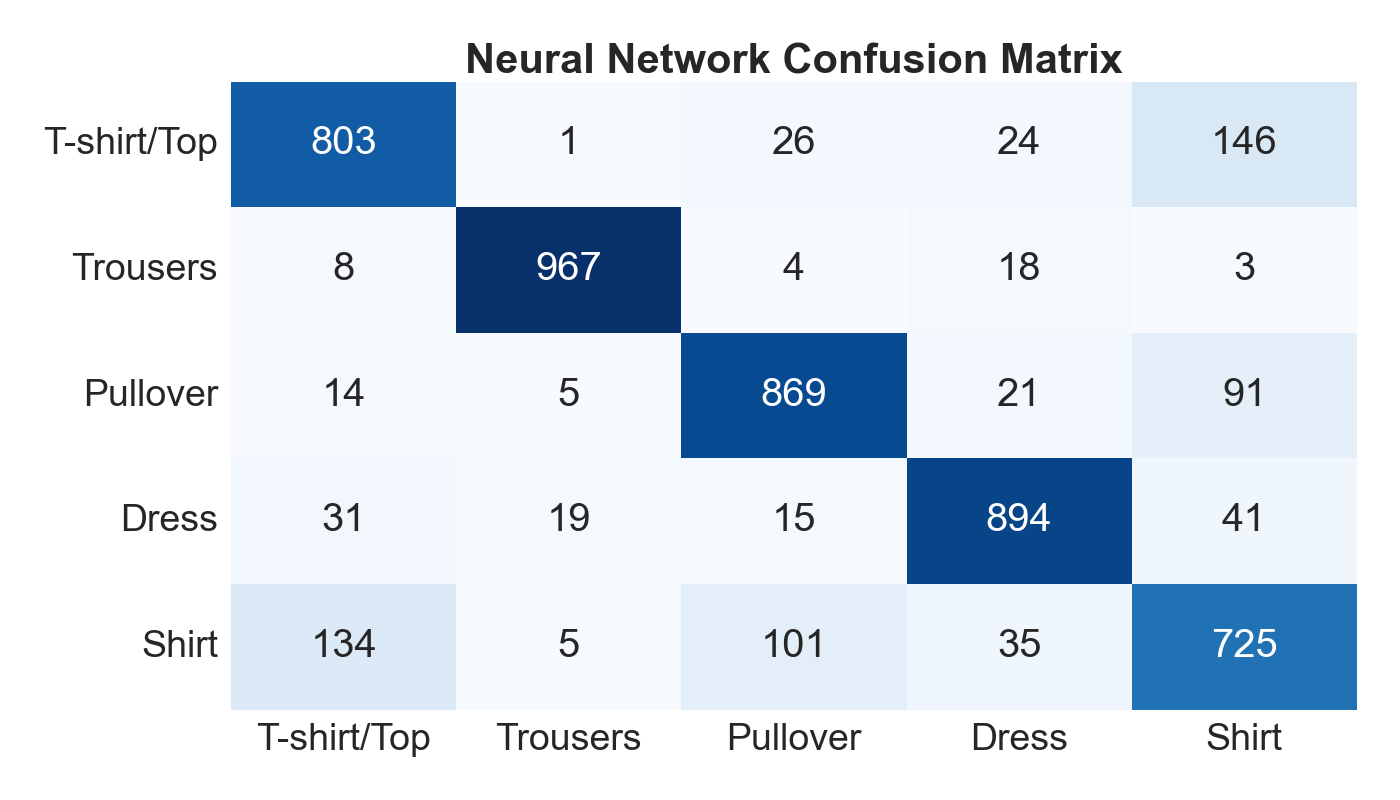
\includegraphics[width=\linewidth]{figures_for_report/Neural Network Confusion Matrix}
  \caption{Neural Network Confusion Matrix}\label{fig:nn_cm}
\endminipage\hfill
\minipage{0.5\textwidth}
  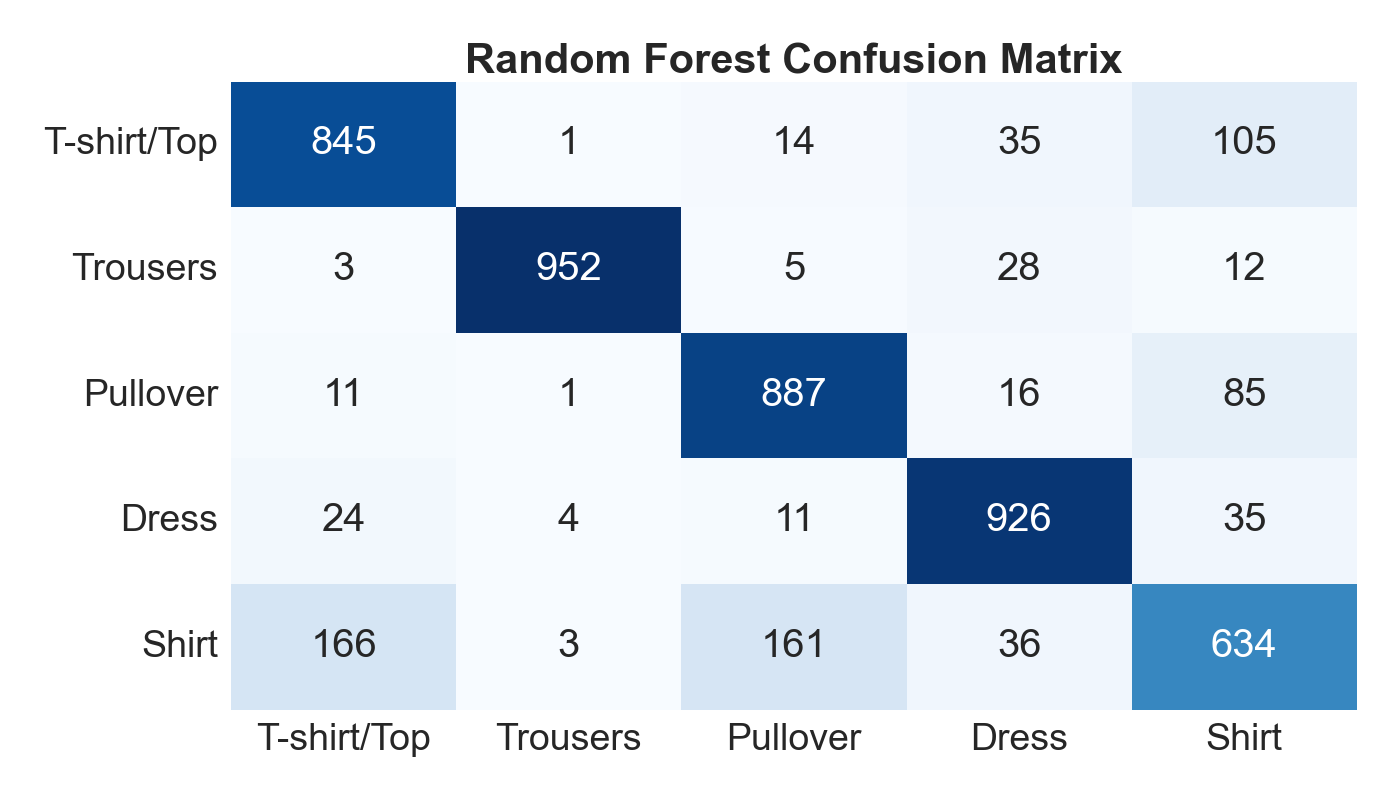
\includegraphics[width=\linewidth]{figures_for_report/Random Forest Confusion Matrix}
  \caption{Random Forest Confusion Matrix}\label{fig:rf_cm}
\endminipage\hfill
    \centering
    \minipage{0.5\textwidth}
  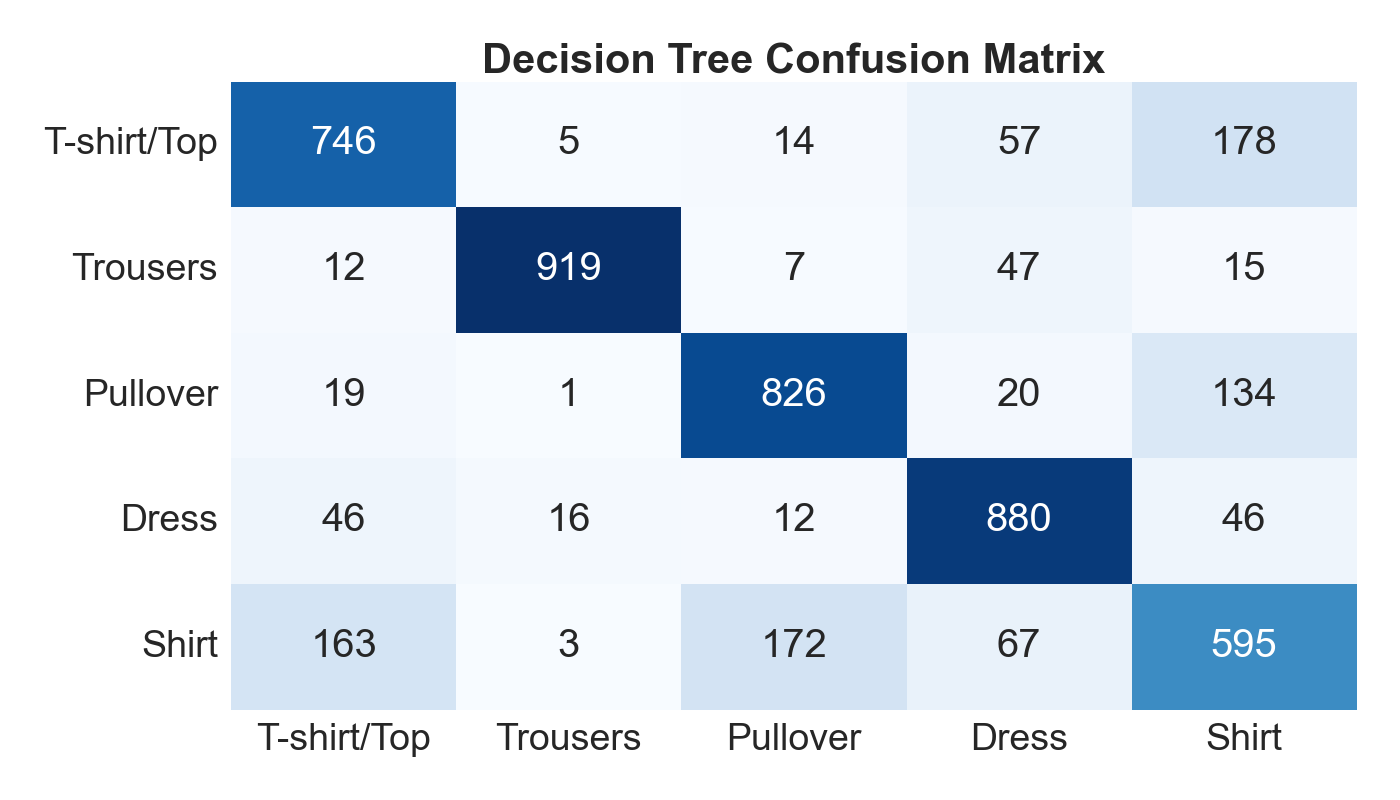
\includegraphics[width=\linewidth]{figures_for_report/Decision Tree Confusion Matrix}
  \caption{Decision Tree Confusion Matrix}\label{fig:dt_cm}
\endminipage\hfill
\end{figure}\label{fig:cfm}

\textbf{Figure 10}, \textbf{11} and \textbf{12}, illustrates the differences in performance across all clothing types for the three classifiers, and illustrates the points made earlier.
The right-most column in the three figures indicates that there is often confusion between the categories Shirts, T-shirts/Tops, and Pullovers.